\section*{\large{ВВЕДЕНИЕ}}

Цель лабораторной работы --- разработать программу шифровальной машины <<DES>> \cite{Enigma}.

Задачи лабораторной работы:

\begin{enumerate}
    \item провести анализ работы шифровальной машина <<DES>>;
    \item описать алгоритм шифрования;
    \item релизовать описанный алгоритм.
\end{enumerate}

\clearpage
\section{Аналитическая часть}

\subsection{Алгоритм шифрования DES}

\textbf{DES} (Data Encryption Standard) \cite{Enigma} --- это симметричный шифровальный алгоритм, разработанный в 1970-х годах, который использует блочное шифрование с фиксированной длиной блока в 64 бита. Вот основные шаги и логика работы DES:

1. \textbf{Начальная перестановка} (Initial Permutation):
Исходный текст (64 бита) проходит через начальную перестановку, где биты переставляются в определенном порядке согласно предопределенной таблице перестановок.

2. \textbf{Раунды шифрования} (Rounds):
DES состоит из 16 раундов шифрования, каждый из которых включает несколько шагов:
\begin{itemize}
	\item[---] \textbf{Расширение} (Expansion): 32-битный входной блок расширяется до 48 бит путем перестановки и дублирования некоторых битов.
	\item[---] \textbf{Ключ раунда} (Round Key): к 48-битному расширенному блоку применяется 48-битный ключ раунда, полученный из основного ключа DES.
	\item[---] \textbf{Скремблирование} (Substitution): 48-битный блок проходит через S-блоки (Substitution-boxes), которые заменяют блоки по 6 бит на блоки по 4 бита с использованием заранее определенных таблиц замен.
	\item[---] \textbf{Перестановка} (Permutation):  после замены, полученный блок по 32 бита проходит через таблицу перестановки, которая перемешивает биты в блоке.
	\item[---] \textbf{Обработка ключа} (Key Mixing): к полученному блоку применяется операция XOR с ключом раунда для обеспечения взаимодействия ключа и данных.
\end{itemize}

3. \textbf{Завершающая перестановка} (Final Permutation):
После 16 раундов, 64-битный блок проходит через последнюю перестановку, обратную начальной перестановке, чтобы получить зашифрованный текст.

Основным элементом DES является ключ, который состоит из 56 бит, и который используется для генерации ключей раунда. Ключ разбивается на две половины, и каждая половина сдвигается влево на определенное количество бит в зависимости от номера раунда. Затем, из полученных половинок формируется ключ раунда.

Таким образом, DES использует комбинацию перестановок, замен и операций XOR для шифрования данных. Эти шаги повторяются 16 раз, в каждом раунде используется уникальный ключ. Результат --- зашифрованный блок данных, который без знания правильного ключа практически невозможно расшифровать.

Алгоритм шифрования DES может использоваться в следующих режимах.

\begin{enumerate}
	\item[1.] \textbf{ECB} (Electronic Code Book) --- режим «электронной кодовой книги» (простая замена);
	\item[2.] \textbf{CBC} (Cipher Block Chaining) --- режим сцепления блоков;
	\item[3.] \textbf{CFB} (Cipher Feed Back) --- режим обратной связи по шифротексту;
	\item[4.] \textbf{OFB} (Output Feed Back) --- режим обратной связи по выходу.
\end{enumerate}

\clearpage

\section{Конструкторская часть}

\subsection{Разработка алгоритма}

На рисунке \ref{fig:algo} представлена схема алгоритма шифрования DES.

%

\begin{figure}[h!]
	\centering
	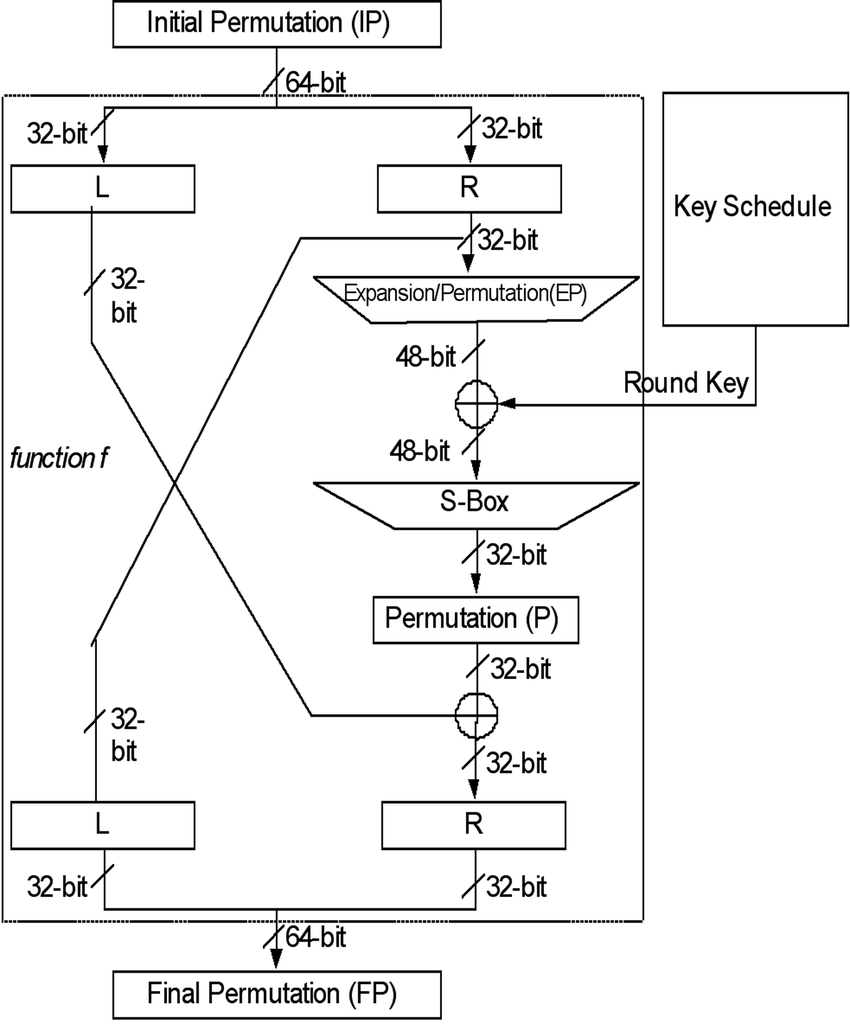
\includegraphics[width=\textwidth]{assets/images/des.png}
	\caption{Схемы алгоритма DES}
	\label{fig:algo}
\end{figure}
\clearpage

\section{Технологическая часть}

\subsection{Средства реализации}

Для реализации ПО был выбран язык C++ \cite{c++}.
В данном языке есть все требующиеся инструменты для данной лабораторной работы.
В качестве среды разработки была выбрана среда VS code \cite{vscode}.

\subsection{Реализация алгоритма}

Реализация PCBC.

\begin{lstlisting}
    void messageBlocksToFile(std::string filenameOut, std::vector<std::vector<int>> messageBlocks, size_t truncateBytesCount) {
        std::vector<std::string> messageBinary;
    
        for (int i = 0; i < int(messageBlocks.size()) - 1; i++) {
            for (int j = 0; j < 8; ++j) {
                std::string curStr;
                for (int s = j * 8; s < messageBlocks[i].size() && s < (j + 1) * 8; s++) {
                    curStr += std::to_string(messageBlocks[i][s]);
                }
                messageBinary.push_back(curStr);
            }
        }
    
        if (!messageBlocks.empty()){
            for (int j = 0; j < 8 - truncateBytesCount; ++j) {
                std::string curStr;
                std::vector<int> block = messageBlocks.back();
                for (int s = j * 8; s < block.size() && s < (j + 1) * 8; s++) {
                    curStr += std::to_string(block[s]);
                }
                messageBinary.push_back(curStr);
            }
        }
    
        std::vector<int> messageOrd;
        for (const auto& x : messageBinary) {
            messageOrd.push_back(std::stoi(x, 0, 2));
        }
    
        std::vector<unsigned char> messageBytes;
        for (const auto& x : messageOrd) {
            messageBytes.push_back(static_cast<unsigned char>(x));
        }
    
        std::ofstream f_out(filenameOut, std::ios::binary);
        for (const auto& x : messageBytes) {
            f_out.write(reinterpret_cast<const char*>(&x), 1);
        }
        f_out.close();
    }    
\end{lstlisting}


\subsection{Тестовые данные}

В таблице \ref{tbl:functional_test} приведены тесты для алгоритма шифрования DES. 
Применена методология черного ящика. Тесты пройдены \textit{успешно}.



\begin{table}[ht!]
	\begin{center}
		\captionsetup{justification=raggedright,singlelinecheck=off}
		\caption{\label{tbl:functional_test} Функциональные тесты}
		\begin{tabular}{|c|c|c|}
			\hline
			Входная строка & Выходная строка \\ 
			\hline
			$ABOBA$ & $BCRGJ$\\
			$BCRGJ$  & $ABOBA$\\
			$<<>>$  & $<<>>$ \\
            $A$ & $T$\\
			$T$  & $A$\\
			\hline
		\end{tabular}
	\end{center}
\end{table}

\clearpage
\section*{\large{ЗАКЛЮЧЕНИЕ}}
В данной лабораторной работе:
\begin{enumerate}
    \item проведен анализ работы шифровальной машина <<DES>>;
    \item описан алгоритм шифрования;
    \item реализован описанный алгоритм;
\end{enumerate}